% Created 2017-10-21 Sat 15:05
% Intended LaTeX compiler: pdflatex
\documentclass[titlepage]{article}
\usepackage[utf8]{inputenc}
\usepackage[T1]{fontenc}
\usepackage{graphicx}
\usepackage{grffile}
\usepackage{longtable}
\usepackage{wrapfig}
\usepackage{rotating}
\usepackage[normalem]{ulem}
\usepackage{amsmath}
\usepackage{textcomp}
\usepackage{amssymb}
\usepackage{capt-of}
\usepackage{hyperref}
\usepackage{mathptmx}
\author{Xiong ChenYu \\
U1521516C \\
EEE \\
}
\date{Oct. 20, 2017 \\
}
\title{
\includegraphics[width=\textwidth]{img/NTU.png} \\
[2\baselineskip] REPORT ON \\
DIGITAL SIGNAL PROCESSING \\
ASSIGNMENT 1 \\
AUDIO EQUALIZER \\
[2\baselineskip]}
\hypersetup{
 pdfauthor={Xiong ChenYu \\
U1521516C \\
EEE \\
},
 pdftitle={
\includegraphics[width=\textwidth]{img/NTU.png} \\
[2\baselineskip] REPORT ON \\
DIGITAL SIGNAL PROCESSING \\
ASSIGNMENT 1 \\
AUDIO EQUALIZER \\
[2\baselineskip]},
 pdfkeywords={},
 pdfsubject={},
 pdfcreator={Emacs 27.0.50 (Org mode 9.1.2)},
 pdflang={English}}
\begin{document}

\maketitle
\tableofcontents

\listoftables
\listoffigures

\newpage
\section{Introduction}
\label{sec:org86ca508}
\subsection{Background}
\label{sec:org8d487b3}
In the information ages everything is store in digital, such as the picture,
the video and the sound. To play the sound from the digital to the
corresponding real analog signal, we need the signal system to do such
things. First we need Software Audio Equalizer to enhance the sound and use a
digital to analog converter to convert the digital to analog with the minimum
noise added in \hyperref[fig:org83e9ed3]{Figure 1} And the last step we need a reconstruction filter to filter out
the high frequency noise and connect to speaker.

\begin{figure}[htbp]
\caption{\label{fig:org83e9ed3}
Audio System}
\centering
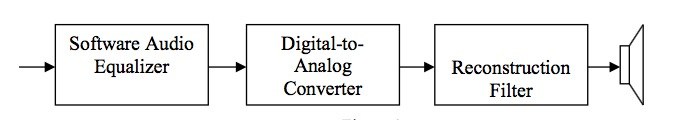
\includegraphics[width=12cm]{./img/audio.png}
\end{figure}

\subsection{Motivation}
\label{sec:orgdb84646}
This semester I take the EE4413 Digital Signal Design, So I learn different
ways to build IIR and FIR filters design to build low/high pass band filter.
Compare to IIR the FIR have linear phase which means FIR is good to design
the sound system without distortion[1].

I decide to build a FIR system to enhance and reduce this 8 bands to get
better music effect as in \hyperref[tab:org3955e82]{Table 1}.
\begin{table}[htbp]
\caption{\label{tab:org3955e82}
Bands}
\centering
\begin{tabular}{rrr}
Band \# & Low & High Frequency(Hz)\\
\hline
1 & 0 & 200\\
2 & 200 & 400\\
3 & 400 & 800\\
4 & 800 & 1600\\
5 & 1600 & 3200\\
6 & 3200 & 6400\\
7 & 6400 & 12300\\
8 & 12300 & 22000\\
\end{tabular}
\end{table}

\subsection{Objective}
\label{sec:org4d9f0cc}

The objective is to design and simulate an audio equalizer using Mat lab by using 512-tap FIR filter structure.

\newpage

\section{Design and system construction}
\label{sec:org807f460}
\subsection{GUI design}
\label{sec:orgd8df49c}

\begin{figure}[htbp]
\caption{\label{fig:org0f31e34}
GUI}
\centering
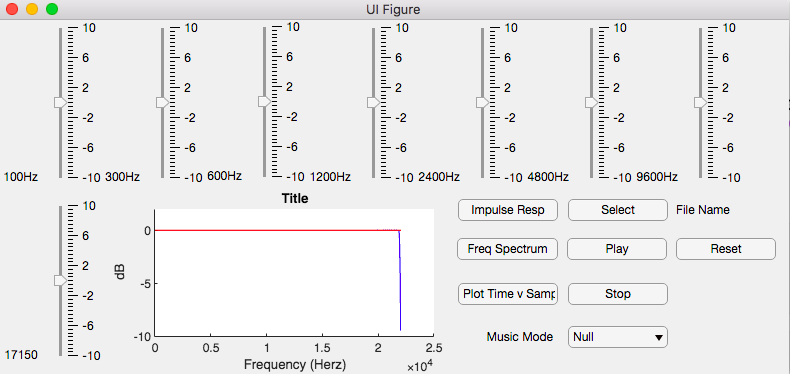
\includegraphics[width=12cm]{./img/1.png}
\end{figure}
For the graphic user interface, I use 8 sliders to control the different
frequency bands. You can find it at \hyperref[fig:org0f31e34]{Figure 2}.

\begin{figure}[htbp]
\caption{\label{fig:org01fa1fb}
Change Slider Value}
\centering
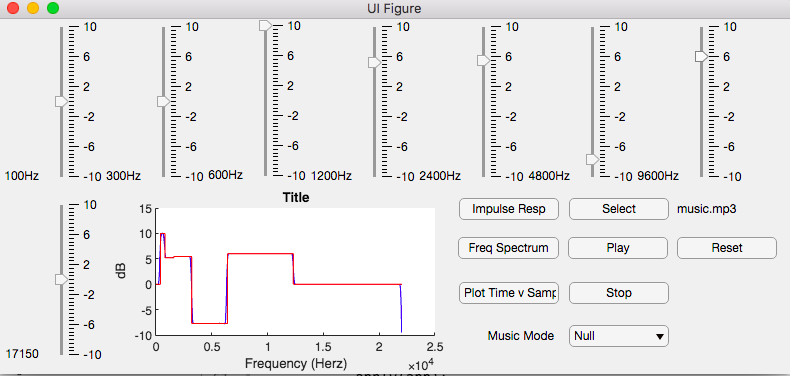
\includegraphics[width=12cm]{./img/3.png}
\end{figure}

The sliders is used to control the different frequency range from -10 DB to
10 DB, and the label show the mid frequency of the band. Every time when I
change the frequency the FIR filter will be automatic regenerate. Like in
\hyperref[fig:org01fa1fb]{Figure 3}.

\begin{figure}[htbp]
\caption{\label{fig:org50f9af5}
Impulse response}
\centering
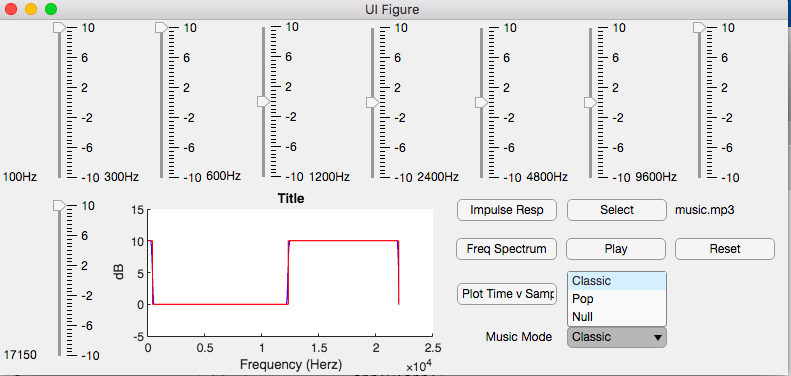
\includegraphics[width=12cm]{./img/5.png}
\end{figure}

In the middle there is a 2-D graph to display the required response and spectrum.
The default graph it the frequency response of the FIR filter and the ideal
frequency response. If you want to see the impulse response in time domain
just click the Impulse Resp button. Then you can get it as in \hyperref[fig:org50f9af5]{Figure 4}.

\begin{figure}[htbp]
\caption{\label{fig:org146612e}
Predefined mode}
\centering
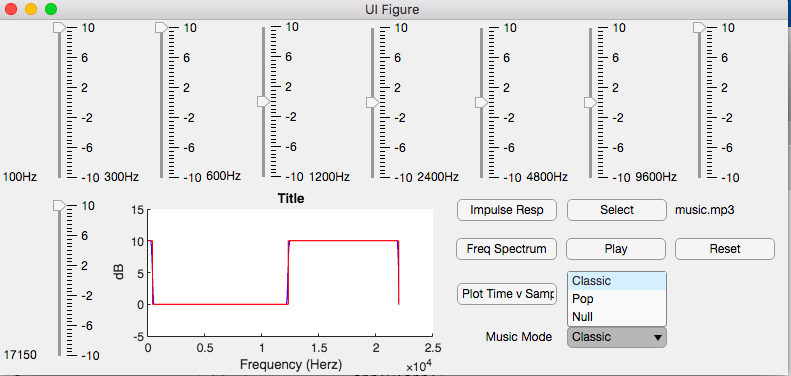
\includegraphics[width=12cm]{./img/5.png}
\end{figure}

On the right side are some control buttons and a select box. For the select
box below there are some predefined filter such as pop music(increase between
500Hz and 4000 Hz). You can choose it and the specified filter will be
applied. As in \hyperref[fig:org146612e]{Figure 5}.

\begin{figure}[htbp]
\caption{\label{fig:orgb9fd908}
Load Digital Data}
\centering
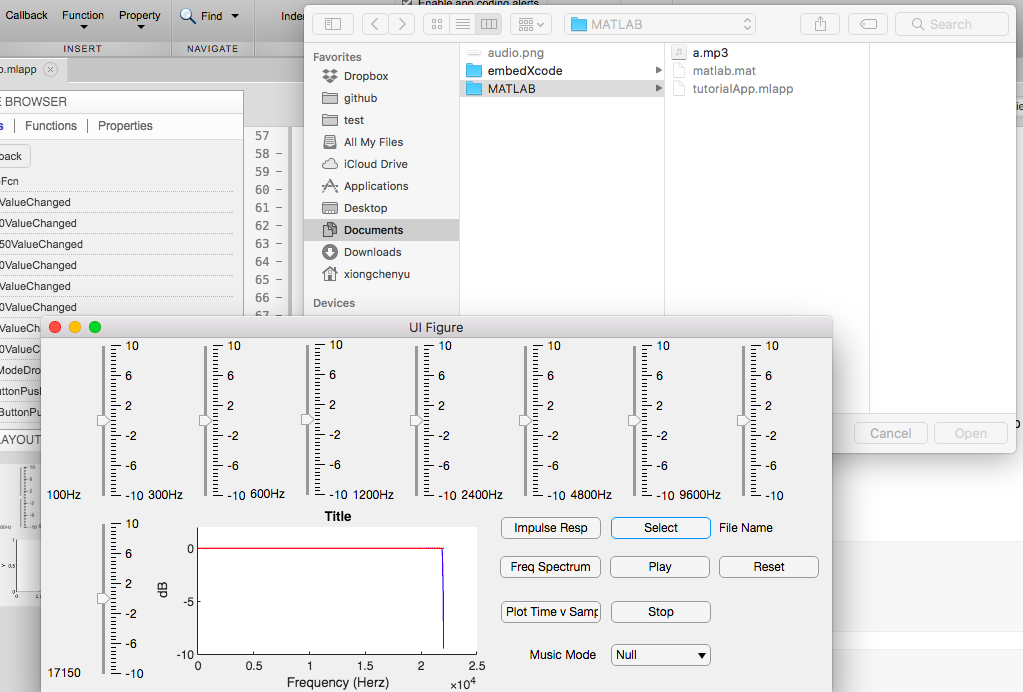
\includegraphics[width=12cm]{./img/2.png}
\end{figure}

After I create the desired FIR filter. I can use the select button
to select a MP3 audio file. Show in \hyperref[fig:orgb9fd908]{Figure 6}. The audio file then will be convert to 2
dimension matrix which stand for the left and right Channel. Then I can use
play button to enjoy the enhanced music.
\begin{figure}[htbp]
\caption{\label{fig:org2a0d4f2}
Frequency Spectrum}
\centering
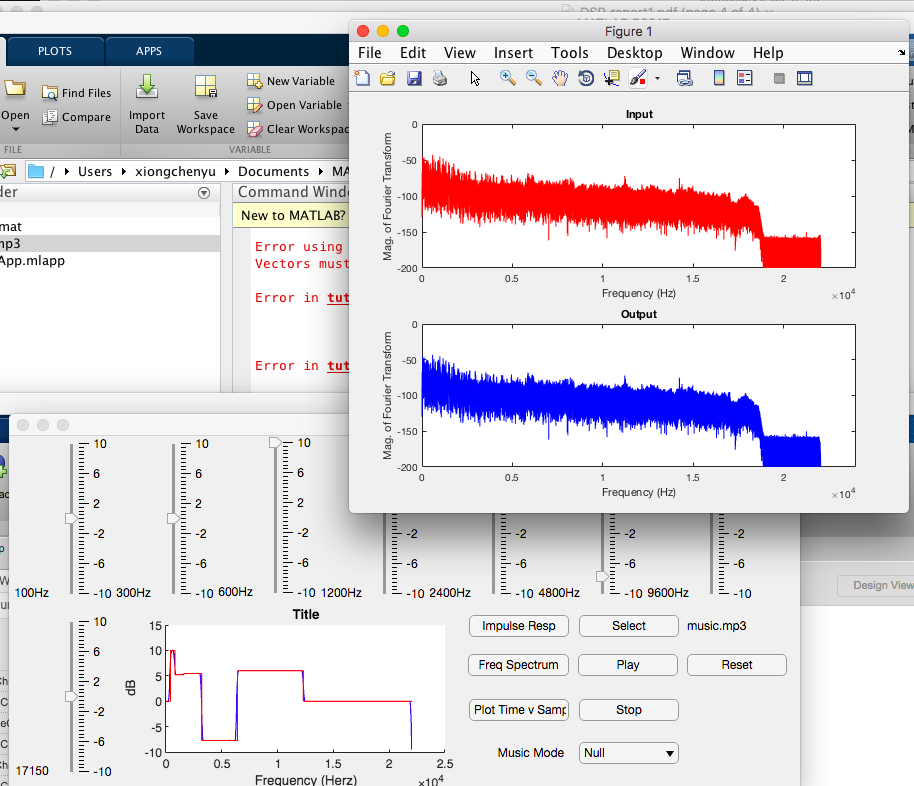
\includegraphics[width=8cm]{./img/4.png}
\end{figure}

\begin{figure}[htbp]
\caption{\label{fig:org085161d}
Data Sample}
\centering
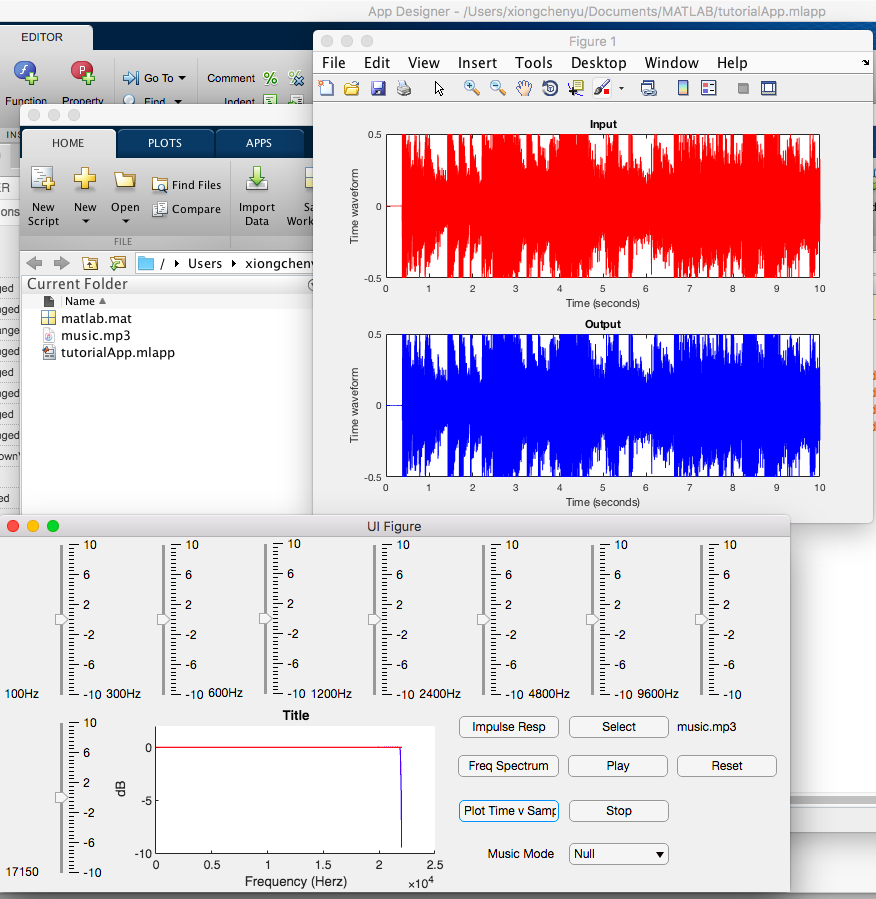
\includegraphics[width=8cm]{./img/7.png}
\end{figure}
I can stop it and analysis the filter. First is to plot the 2 frequency
spectrum of the origin and filtered data as in \hyperref[fig:org2a0d4f2]{Figure 7}. And also the first 10 second data
samples of the input and output. As in \hyperref[fig:org085161d]{Figure 8}.

\subsection{System Construction}
\label{sec:org6a89275}
The system is configured by change the sliders to control the gain. And load
digital signal by choose a MP3 file to get input. First you should make a
desired gain by each frequency range, and the coefficient will be auto
calculated, then you can choose a music by the time you select the music the
filtered data will be automatic generate by the filter. Then you can play the
filter signal and stop it, what's more you can easily analysis it.

\section{Algorithm and simulation}
\label{sec:org5faee99}
The frequency response of ideal FIR filter is the block wave, but it is
unrealistic to compute in the computer because the reverse fourier transform
of a squire block is \(sinc\) which is infinite in time domain. One of the most
famous way is to use window function in this infinite impulse response trim
the transfer CCDE to finite then do fourier transform to the CCDE trimmed by
window function. The window function is strait forward and can easy design
simple high/low/band pass/stop filters. But this method is complicated to
design an arbitrary filter here.

Luckily, matlab offers a great FIR function fir2 which use the frequency
sampling design method. Below shows the algorithms of frequency sampling
method. See \hyperref[fig:org92060a0]{Figure 9}.

\begin{figure}[htbp]
\caption{\label{fig:org92060a0}
Frequency Sampling Method}
\centering
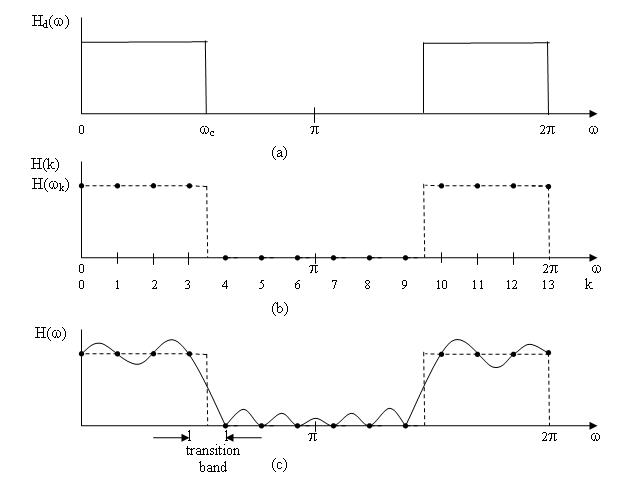
\includegraphics[width=12cm]{./img/14.jpg}
\end{figure}

$$ H_d(e^j\omega) \Rightarrow H_d(K) \Rightarrow h(n) $$
$$ \omega = \frac{2{\pi}k}{N} $$

Then we can use IDFT to get the transfer function h(n).

$$ h(n) = \frac{1}{N}\sum_{k=0}^{N-1}H_d(k)W_N^{(-nk)}$$

  Since the tap is 512 so the order of the filter is 512 -1 = 511. So the value
511 is odd To ensure the coefficient of h(n) is always real. We can use the
equation below[2] to get the real h(n).
$$ h(n) = \frac{1}{N}[H(0) + 2\sum_{k=1}^{\frac{N-1}{2}}Re(H(k)e^\frac{j2{\pi}an}{N})] $$

So we can get the real h(x) coefficient by frequency sampling method.

The simulation can be seen in \hyperref[fig:org146612e]{Figure 5.}

\begin{figure}[htbp]
\caption{\label{fig:org3c5c511}
Maximum of origin data and filtered data}
\centering
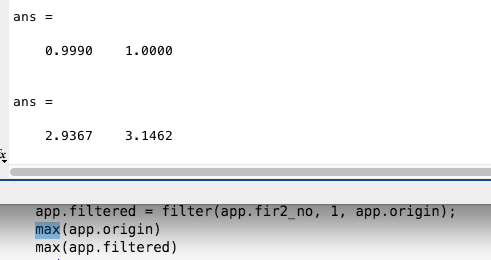
\includegraphics[width=12cm]{./img/9.png}
\end{figure}

You can see from \hyperref[fig:org3c5c511]{Figure 10}. The maximum of the MP3 amplitude is 1, and the
maximum of data filtered is 3.1. To prevent the possibility of signal clipping,
normalize the filtered signal before it is output to the DAC. Rather than use
normal \textbf{sound} function. I use \textbf{soundsc} function to normalize the date before
play it. soundsc(y) scales the values of audio signal y to fit in the range from
–1.0 to 1.0, and then sends the data to the speaker at the default sample rate
of 8192 hertz. By first scaling the data, soundsc plays the audio as loudly as
possible without clipping. The mean of the dynamic range of the data is set to
zero. [3]

\section{Results, analysis and discussion}
\label{sec:orgd9f12fc}
To analysis the result, first we need to compare the input and output sample data
when gain equal to 0 DB. And it is the same in \hyperref[fig:org2a0d4f2]{Figure7}.
\begin{figure}[htbp]
\caption{\label{fig:org74f4b11}
Classic Frequency Response}
\centering
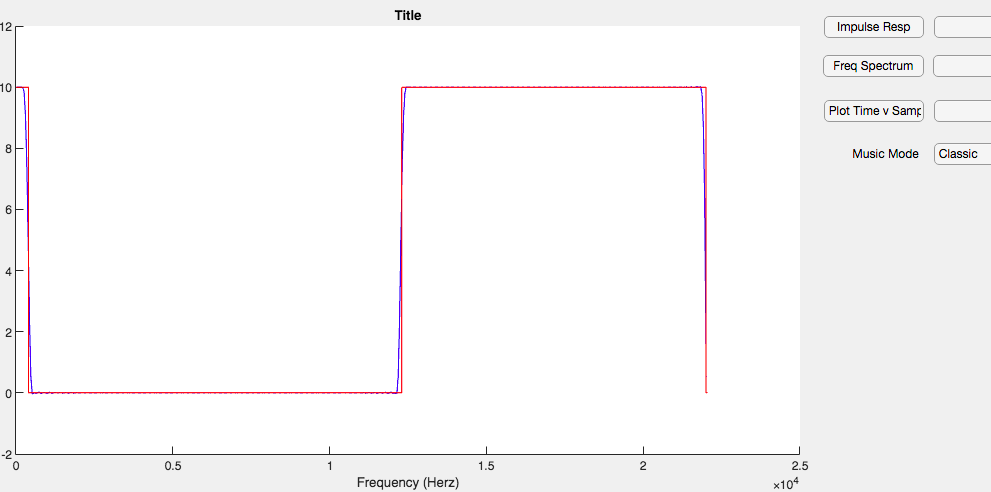
\includegraphics[width=12cm]{./img/10.png}
\end{figure}

\begin{figure}[htbp]
\caption{\label{fig:org7951797}
Classic Impulse Response}
\centering
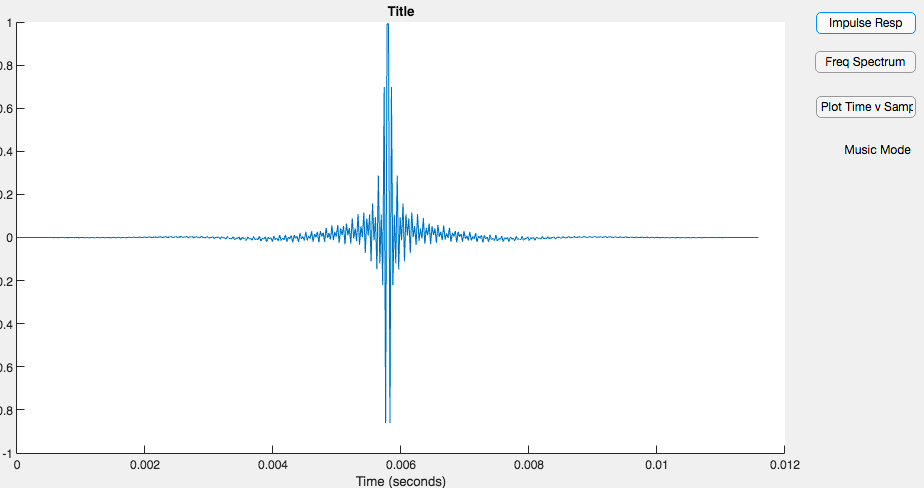
\includegraphics[width=12cm]{./img/11.png}
\end{figure}

\begin{figure}[htbp]
\caption{\label{fig:orgcbffb77}
Pop Frequency Response}
\centering
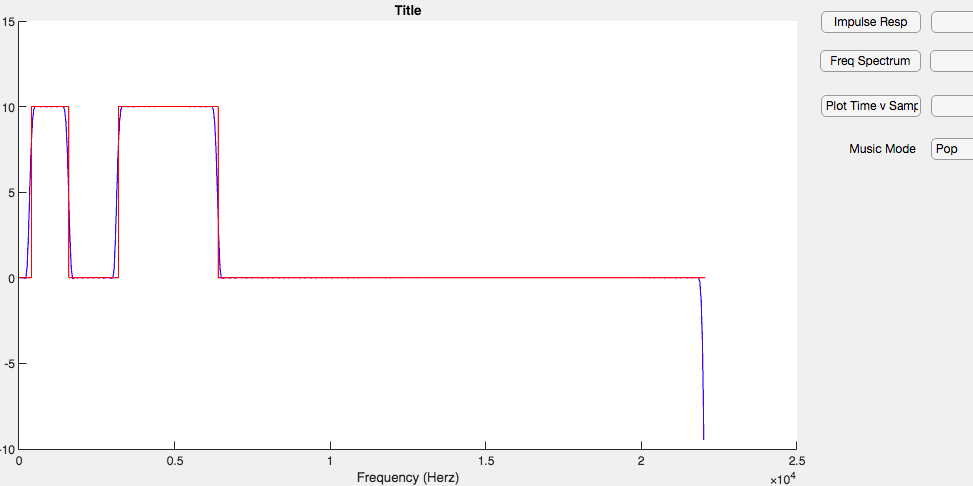
\includegraphics[width=12cm]{./img/12.png}
\end{figure}

\begin{figure}[htbp]
\caption{\label{fig:orgcf5dc85}
Pop Impulse Response}
\centering
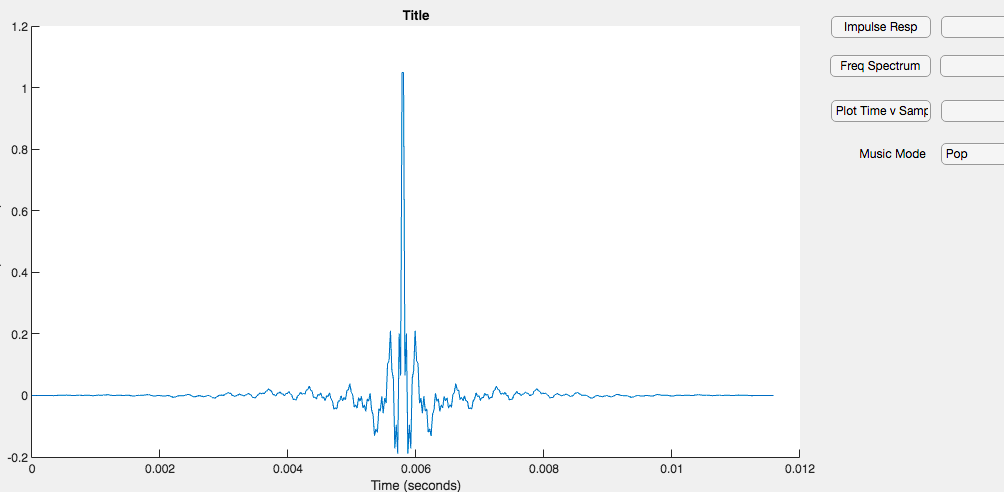
\includegraphics[width=12cm]{./img/13.png}
\end{figure}

And let us analysis the 2 condition classic music filter and pop music filter.
First let us see the frequency response at \hyperref[fig:org74f4b11]{Figure 11} and \hyperref[fig:orgcbffb77]{Figure 13.}
The red line stand for the ideal FIR filter and the blue line is the actual
filter. You can see the real FIR filtered transition edge is a vertical line
which means it pass band equal to stop band. Transition band equal to 0. And
for the real FIR the transition band at high frequency is larger than the
transition band in low frequency.

As for the impulse response \hyperref[fig:org7951797]{Figure 12} and \hyperref[fig:orgcf5dc85]{Figure 14}. For the classic filter
which enhance the high frequency the frequency of the wave is high while the
pop filter frequency is low. And since the classic filter enhanced the
frequency below 500Hz and above 4000Hz. The pop filter enhance the frequency
between 500Hz and 4000Hz. So the filter is orthogonal there wave can cancel
each other out. So the impulse response of classic music filter and pop music
filter add together is the impulse function.

\section{Conclusions and recommendations}
\label{sec:org85caf75}
This Frequency sampling method designed FIR filter is good and works well but
there are some other good design method can be implement.

I just try the frequency sampling method in this report and use hamming
function, I the future can try some other window function to decrease the
signal leakage.

I also recommend to use all kind of design method such as Window design
method, Weighted least squares design, Parks-McClellan method etc. To compare
the similarity and difference.



\addcontentsline{toc}{section}{References}

  \begin{thebibliography}{99}

  \bibitem{1}\textsc{En.wikipedia.org}\texttt{.(2017). Finite impulse response. [online] Available at:
  https://en.wikipedia.org/wiki/Finite_impulse_response
[Accessed 20 Oct. 2017].}

  \bibitem{2}\textsc{YouTube}\texttt{.(2017). How to Design FIR FIlters using frequency sampling method.
[online] Available at: https://www.youtube.com/watch?v=O0DbpZqhPSg [Accessed 20 Oct. 2017].}

  \bibitem{3}\textsc{Mathworks.com}\texttt{
[online] Available at: https://www.mathworks.com/help/matlab/ref/soundsc.html?searchHighlight=soundsc&s_tid=doc_srchtitle [Accessed 20 Oct. 2017].}

\end{thebibliography}
\end{document}